\subsection{Experiments}\label{subsec:rupture_experiments}

In this section we provide results on various experiments we conducted in lab
environment to evaluate the performance of Rupture. These results reflect
Rupture's versatility when it comes to attacking different protocols and are a
good basis in order to evaluate the tool against real-world systems in future
work.

Our lab environment consisted of a single web page which is hosted on an Nginx
web server. This page contains digits and a single word, which consists of 8
lowercase English letters and serves as the secret. The first two characters of
the word are known and were used in order to bootstrap the attack. It also
offers a GET URL parameter and reflects the parameter's value in the middle of
the digits of the page. This page is the most basic scenario for a BREACH
attack, since it is noiseless and the secret's alphabet is different from the
rest of the page, thus avoiding cross-compression issues.

We deployed all Rupture modules on a single machine and used this same machine
as a victim, so there was no need for injection.

We utilized most optimizations proposed in the previous sections. We used a
permutation of all uppercase English letters for the block alignment,
issued 32 requests in parallel for each character candidate in the form of a
soup, and used the serial method for computing the reflection strings.

Figure \ref{fig:rupture_performance_aes_gcm} shows the results of our
experiments against the AES algorithm in GCM mode for block sizes of 128 and 256
bits.

   \begin{figure}[thpb]
      \centering
          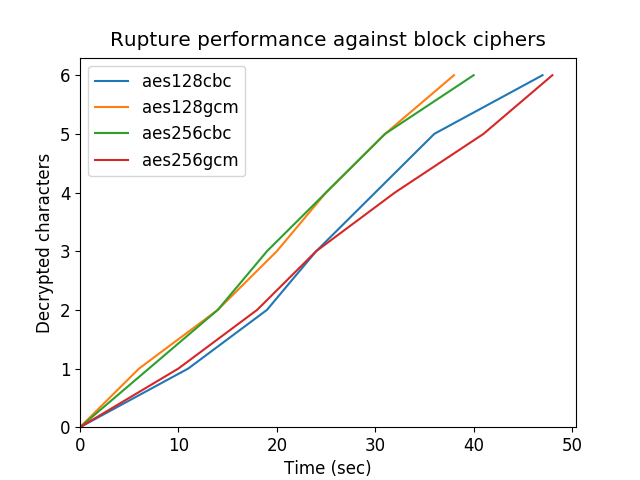
\includegraphics[width=0.48\textwidth]{experiments/rupture_performance/rupture_performance.png}
      \caption{Rupture performance against AES GCM mode}
      \label{fig:rupture_performance_aes_gcm}
   \end{figure}

We were able to consistently decrypt all 6 unknown characters of the word in
both cases. In the case of 256-bit blocksize, we decrypted the characters in
167 seconds, which amounts to roughly 27 seconds per character. In the case of
128-bit blocksize, the attack lasted 245 seconds, which is about 40 seconds per
character. However, in this case we should observe the long amount of time that
was needed to decrypt the final character. This occured because Rupture needed
more request sets in order to build enough confidence on its choice compared to
the other characters.
